% *******************************************************************************
% * Copyright (c) 2007 by Elexis
% * All rights reserved. This document and the accompanying materials
% * are made available under the terms of the Eclipse Public License v1.0
% * which accompanies this distribution, and is available at
% * http://www.eclipse.org/legal/epl-v10.html
% *
% * Contributors:
% *    G. Weirich - initial implementation
% *
% *  $Id: stammdaten.tex 4911 2009-01-05 17:56:39Z rgw_ch $
% *******************************************************************************
% !Mode:: "TeX:UTF-8" (encoding info for WinEdt)

\section{'Views' des données de base}

\subsection{patients}
\index{Liste des patients}
La liste des patients affiche les données saisis des patients mais sert aussi pour la saisie des nouvelles entrées. La liste affiche tous les contacts qui sont marqués comme 'patient'.
\begin{figure}[ht]
	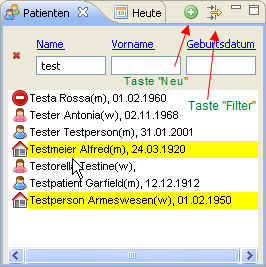
\includegraphics{images/patlistview}
	\caption{Patientenliste}
	\label{fig:patlist}
\end{figure}

Les champs de saisie en haut (nom, prénom, date de naissance) servent à limiter la liste conformément aux paramètres souhaités.
\begin{itemize}
  \item S'applique pour le nom et prénom :
	\begin{itemize}
      \item Si vous suggérez au moins deux lettres, il n'apparaîtront sur la liste que les entrées qui \textit{commencent} avec ces deux lettres.
      \item Lorsque vous introduisez le signe % et au moins deux autres lettres, les entrées qui \textit{contiennent}cette séquence de caractères apparaîtront sur la liste.
    \end{itemize}
  \item S'applique pour la date de naissance :
	\begin{itemize}
      \item Lorsque vous suggérez au moins 3 chiffres successifs les chiffres sont interprétés comme année et les patients qui ont \textit{l'année de naissance } correspondante seront affichés.
      \item Si vous introduisez deux chiffres, suivi d'un point et évtl. d'autres 2 chiffres, les patients avec cette \textit{date de naissance } (jour) et évtuellement \textit{le mois de naissance } correspondant s'afficheront.
      Veuillez considérer que vous devez introduire le jour et le mois toujours à deux chiffres, donc p. ex. 04.05. et non 4.5.
     \end{itemize}
\end{itemize}
S'il n'y a pas de données saisies qui correspondent aux conditions du filtre l'affiche : \glqq pas de données\grqq apparaîtra sur la liste.

\medskip
\index{Patient No} \index{Liste des patients!filtrer}
Vous pouvez influencer les champs des filtres correspondants par un préréglage (cf \ref{userconfig} page \pageref{userconfig}).

\subsubsection{Marquage / Stickers}
\index{patients!marquer}\index{patients!marquer}
Vous pouvez influencer l'affichage de la saisie des patients au moyen de certains critères.
Nous appelons ici cette technique des 'Stickers'. Chaque patient peut avoir zéro à plusieurs 'Stickers' qui peuvent alors apparaître dans la liste des patients aussi bien que dans les notes de la consultation. Vous trouvez des indications plus précises sous  \ref{Etiketten} à la page \pageref{Etiketten};

\subsubsection{Barre d'outils}
\begin{itemize}
  \item Par la touche  \glqq New\grqq{}(bouton vert avec croix blanche)  (cf Fig. \ref{fig:patlist}) vous pouvez saisir un nouveau patient. La boîte de dialogue pour l'introduction des nouveaux patients s'ouvre, si vous cliquez sur ce bouton. Les champs que vous avez déjà remplis y apparaissent et vous pouvez introduire les autres données telles qu'elles sont actuellement connues. En cliquant sur \glqq OK\grqq{}la nouvelle entrée du patient est crée. Si vous cliquez sur\glqq fermer\grqq{}les données sont rejetées et aucune nouvelle entrée est faite. Une demande de précisions apparaîtra si une nouvelle entrée doit être faite lorsqu'une entrée avec les mêmes données existe déjà.



  \item Par la touche  \glqq filtre\grqq{} (cf Fig. \ref{fig:patlist}) vous pouvez ouvrir ou fermer une boite de dialogue pour filtrer la liste selon des différentes critères (cf  Fig. \ref{fig:patlistfilter}).
	\begin{figure}[ht]
        \begin{minipage}{0.5\textwidth}
        \centering
    	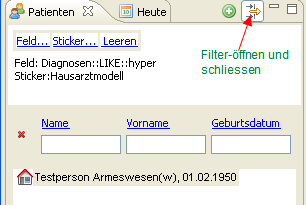
\includegraphics[width=0.8\textwidth]{images/patlistfilter}
    	\caption{Filterbox öffnen}
    	\label{fig:patlistfilter}
        \end{minipage}\hfill
        \begin{minipage}{0.5\textwidth}
        \centering
        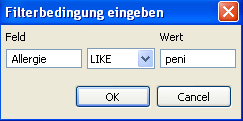
\includegraphics[width=0.8\textwidth]{images/patlistfilter2}
        \caption{Filterausdruck}\label{fig:filterexpr}
        \end{minipage}
    \end{figure}
\end{itemize}

Vous pouvez influencer le filtrage de différentes manières :
\begin{itemize}
\item Si vous cliquez sur 'le champ…' une boîte de dialogue s'ouvre comme dans la Fig. \ref{fig:filterexpr}. Vous pouvez interroger ici des champs de base de données de façon arbitraire. Le '=' signifie : la terminologie doit être exactement la même y inclus l'écriture en majuscule ou minuscule. ' LIKE' signifie : L'expression doit commencer ainsi mais l'écriture en majuscule ou minuscule ne joue aucun rôle.  ' REGEXP signifie: L'expression doit être interprétée comme un terme fixe. Une explication de ce concept conduirait ici toutefois trop loin.


\item Lorsqu'on clique sur 'Sticker' une boite de dialogue s'ouvre qui contient tout les stickers qui sont définis dans le système. Vous pouvez en choisir un ou même plusieurs.
\item Vous pouvez aussi tirer par Drag and Drop un script qui se trouve dans 'script-view' dans le champs de filtrage ce qui permet de calculer des conditions au choix. (cf \ref{Script} à la page \pageref{Script}.
\end{itemize}

Les conditions de filtre sont traitées strictement d'en haut vers le bas. L'expression de filtre
suggérée en deuxième ligne n'est ainsi évaluée que lorsque la première a été passé. Il est donc judicieux d'utiliser des filtres moins intensifs de point de vu calcul (p. ex. Sticker) en haut et ceux qui sont plus intensifs plus bas.(p. ex. Scripts). Cliquez alors sur une des têtes de colonne ou sur 'le x', pour lire la liste -
cette fois-ci sous l'influence des filtres.


\medskip

Pour éliminer une condition de filtre, cliquez la touche droite et choisissez 'éliminer'. Pour éliminer tout, cliquez sur' vider'. Pour mettre le filtre seulement temporairement hors circuit, sans vouloir le vider, cliquez simplement sur le bouton de filtre.


\subsubsection{Menu contextuel}
Le menu contextuel apparaît lorsque vous cliquez avec la touche droite de la souris sur une saisie d'un patient. Il contient les possibilités suivantes :
\begin{itemize}
    \item Sticker … ainsi vous pouvez attribuer un sticker à ce patient ou l'éliminer (cf \ref{Etiketten}).
  \item Effacer le patient (voir ci-dessus)\footnote{pour cela vous nécessitez l'autorisation \textsc{effacer/contact} (cf \ref{sec:gruppen})}
  \item Exporter dossier. Si un Plugin d'exportation est installé ceci permet l'exportation du dossier médical du patient actuellement marqué. Si plusieurs Plugins d'exportation existent il y apparaît une boite de dialogue où on peut choisir la destination et le format\footnote{pour cela vous nécessitez l'autorisation \textsc{fichier/contact/exporter}}
\end{itemize}


\subsection{Patients - détail}
\index{patient!détail}
Cette 'View' (Fig. \ref{fig:patdetail} montre des détails du patient momentanément choisi. 
 %\usepackage{graphics} is needed for \includegraphics

\begin{figure}[t]
\centering
  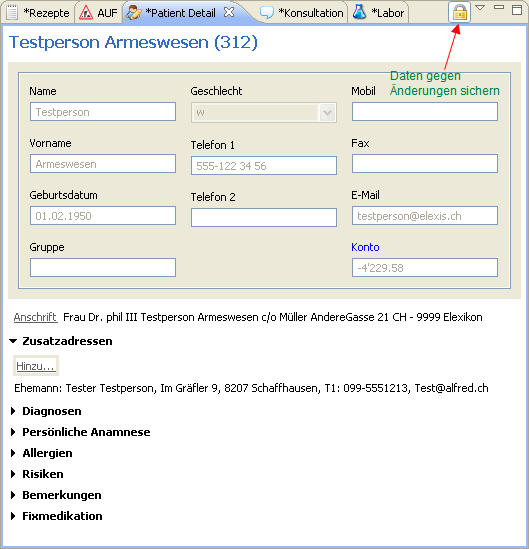
\includegraphics[width=0.8\textwidth]{images/patdetail}
  \caption{Patient Detailansicht}
  \label{fig:patdetail}
  \hfill

\end{figure}

Vous voyez que les différents données saisies apparaissent de couleur grise et ne peuvent pas être modifiées. Si vous cliquez sur le symbole de cadenas à droite en haut, vous pouvez débloquer cette 'View' (si vous possédez les droits correspondants). Ensuite les données de tous les champs peuvent être changées en les écrasant par des nouvelles. Une modification est sauvegardée au moment qu'on quitte un champ. (Le stockage explicite n'est jamais nécessaire dans Elexis). Lorsque vous cliquez de nouveau sur le cadenas ou lorsque vous choisissez un autre patient, la protection se remet en action pour éviter que vous écrasiez des données par erreur.

\medskip

Les champs dans le bloc supérieur sont tous des champs de texte d'une seule ligne et peuvent être modifiés directement à part du champ \glqq compte\grqq{}, qui n'est pas directement réinscriptible. Ce champ affiche le solde de toutes les factures du patient. Si l'utilisateur actuellement inscrit possède les droits d'accéder à la facturation, il peut cliquer sur le texte bleu \glqq compte\grqq{} ce qui ouvre un dialogue dans lequel les différentes payements peuvent être comptabilisés.

\textbf{ATTENTION}: Les écritures se font normalement de façon automatique par la facturation
et l'enregistrement des 'fichiers ESR'. Des écritures manuelles peuvent conduire à des contradictions dans la comptabilité. Ne faites donc des écritures manuelles que lorsque vous êtes conscient des conséquences des changements que vous faites.


 Le champ\glqq adresse\grqq{} indique l'adresse postale du patient.\footnote{L'adresse postale est ce qui apparaît sur les enveloppes et les étiquettes d'adresses. Celle-ci ne doit pas forcément être identique aux données d'adresses introduites. Il peut y apparaître par ex. en plus c/o, cp ou personne de contact} . Celle-ci peut être modifiée en cliquant sur le texte bleu \glqq adresse \grqq{}.

Les champs situé en dessous peuvent tous être ouverts : Normalement seul les titres sont visible et les champs s'ouvrent en cliquant sur le titre.
\begin{itemize}
  \item Le champ \glqq adresses supplémentaires\grqq{}permet de saisir les contacts qui sont en
relation avec un patient. Par exemple membres de famille, offices, d'autres médecins etc. En cliquant sur\glqq ajouter\grqq{} on ouvre une boîte qui contient des différents contacts où on peut choisir ou introduire la personne ou l'organisme en question. Ensuite une autre boîte s'ouvre, dans laquelle les relations du contact choisi avec le patient peuvent être décrites.\\
  Par un clic droit sur une entrée dans ce champ, un menu de contexte s'ouvre qui permet d'afficher out d'éliminer l'entrée entière.
  \item On peut introduire des données dans les champs \glqq Diagnostic\grqq, \glqq Anamnèse personelle\grqq{},
  \glqq Allergies\grqq{}, \glqq Risques\grqq{} und \glqq Remarques\grqq{} lesquelles seront sauvegardées immédiatement lorsqu'on quitte le champ.
  \item Le champ \glqq Médication fixe\grqq{}correspond à la 'View' de la médication fixe.

\end{itemize}
\subsection{Contacts}
Cette 'View' (Fig. \ref{fig:kontaktlist}) montre une liste de tout les contacts introduits dans Elexis. Un contact est chaque personne ou organisation qui a un rapport quelconque avec le cabinet médical. Il s'agit par exemple des patients, collègues, hôpitaux, assurances, laboratoires, fournisseurs etc. 
%\usepackage{graphics} is needed for \includegraphics
\begin{figure}[htp]
\begin{center}
  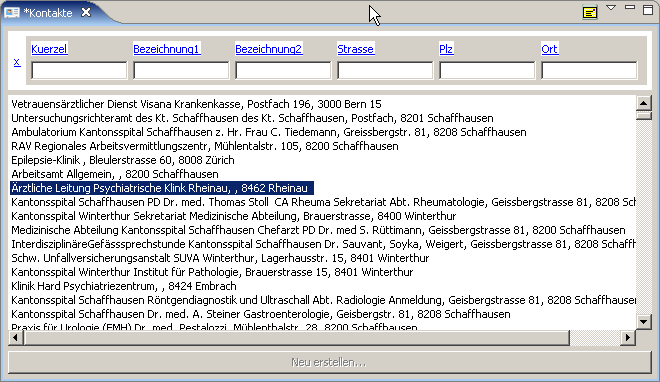
\includegraphics[width=0.9\textwidth]{images/kontaktlistview}
  \caption{Kontaktliste-View}
  \label{fig:kontaktlist}
\end{center}
\end{figure}
En cliquant sur le symbole de l'enveloppe à droite en haut, vous pouvez imprimer une étiquette avec l'adresse du contact choisi.

\subsection{Contacts - détail}
Ici, les détails du contact sélectionné sont indiqués et peuvent être modifiés (Fig. \ref{fig:kontaktdetail}).
%\usepackage{graphics} is needed for \includegraphics
\begin{figure}[htp]
\begin{center}
  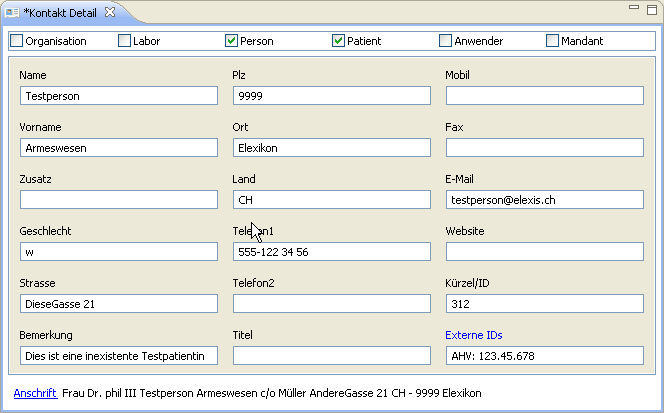
\includegraphics[width=0.9\textwidth]{images/kontaktdetail}
  \caption{Kontakt Detailview}
  \label{fig:kontaktdetail}
\end{center}
\end{figure}
Dans les Checkboxes de la ligne supérieure, vous pouvez définir le type de contact en question. Prenez en considération qu'un contact peut aussi avoir plusieurs types (quelqu'un peut par exemple être utilisateur et également patient ). Par contre un contact ne peut seulement être soit une organisation soit une personne. Veillez également d'introduire ceci correctement. Pour des personnes il ne faut pas oublier de saisir le sexe (m ou f), puisque des modèles de formatage de texte utilisent ces informations pour choisir des formules correctes.

\medskip

Le champ 'sigle/ID' contient sous patients le numéro du patient et ne doit pas être changé. Pour d'autres contacts il peut être utile de définir un sigle spécifique pour pouvoir les trouver plus facilement . Par exemple on peut introduire des médecins avec le préfixe 'méd' suivi de la spécialité et des initiales. Pour les assurances ceci pourrait être le préfix 'ass' etc. L'interniste Docteur Ernst Meier serait à trouver par ex. sous : médIntEM.
L'assurance SWICA à Schaffhouse sous : assSwicaSH.
Les inscriptions ne doivent pas forcément être sans équivoque et on n'est pas forcé d'utiliser ce gadget mais il peut simplement être utile pour rapidement trouver les adresses lorsqu'on doit écrire une lettre.

\medskip

 Le champ'ID externe' sert à établir une quantité arbitraire d'identifications (XID) reçus de l'extérieur. En cliquant sur 'ID externe' de couleur bleue on ouvre un champ de dialogue dans lequel se trouvent toutes les identifications externes déjà existantes. Dans la 'View - contact - détails' on trouve toujours la 'meilleure' càd l'identification la plus sure qui est sans équivoque. Des exemples pour une XID sont le code EAN, le numéro de l'OFSP, des numéros d'assurance sociale/AVS etc.

\medskip

L'adresse postale du contact en question se trouve dans la dernière ligne. Il s'agit de l'adresse, comme elle doit apparaître par exemple dans la zone d'adresse des lettres ou des factures ou sur des étiquettes d'adresse. Cliquez sur le mot en bleu \glqq adresse\grqq{}et la boîte de dialogue d'entrée d'adresse s'ouvre. (Fig.
\ref{fig:anschrift}), où vous pouvez introduire un texte quelconque.  (En cliquant sur le bouton \glqq adresse postale \grqq{} vous créez une adresse standard basée sur les indications des adresses existantes).



\begin{figure}[htp]
\begin{center}
  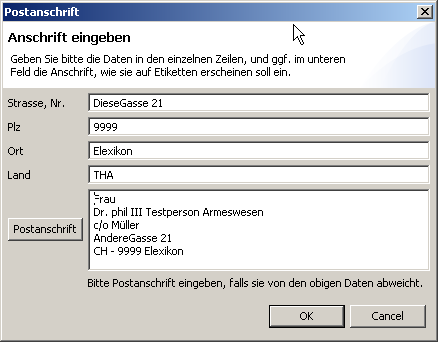
\includegraphics{images/anschrifteingabe}
  \caption{Anschrift-Eingabe}
  \label{fig:anschrift}
\end{center}
\end{figure}
\bigskip
\pagebreak[3]
\subsection{Artikel}
\label{view:artikel}
\index{Article}
Tout objet qui peut être stocké ou / et être remis au patient est un \glqq article\grqq{}. D'un côté ils y existent des articles prédéfinis (par ex. liste de tout les médicaments admis), de l'autre ils y existent aussi des produits propres. Elexis peut administrer le stock des produits et effectuer des commandes de façon semi-automatique pour des articles dont le stock est en train de s'épuiser.


\subsection{Listing des articles}
La Fig. \ref{fig:artikel} montre une liste de sélection d'article et la représentation détaillée des articles.

 %\usepackage{graphics} is needed for \includegraphics
\begin{figure}[htp]
\begin{center}
  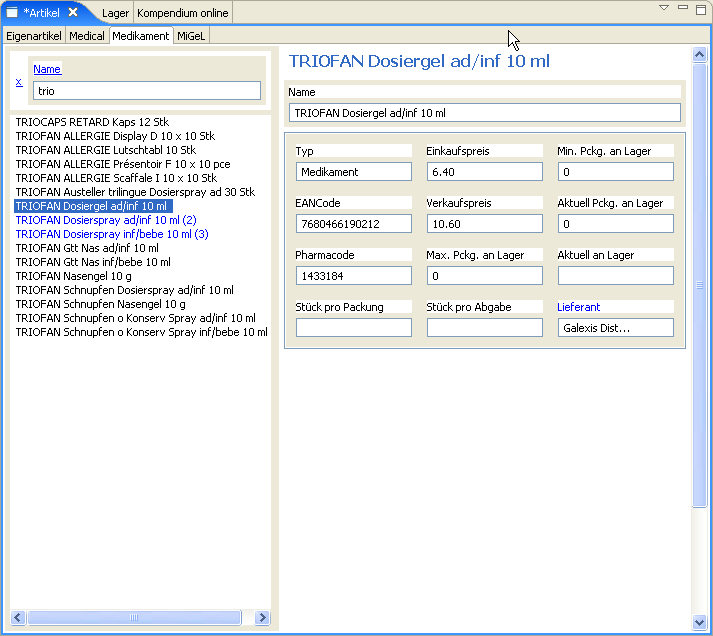
\includegraphics[width=0.9\textwidth]{images/artikelview}
  \caption{Artikel-View}
  \label{fig:artikel}
\end{center}
\end{figure}
Vous pouvez filtrer la liste à gauche de façon habituelle en introduisant les premières lettres du nom de l'article recherché. Vous pouvez voir les détails de l'article sélectionné dans la représentation détaillée. (Dans des perspectives où seulement la liste est représentée, vous pouvez accéder à l'aperçu détaillé en appuyant sur la touche droite de la souris et en choisissant  \glqq modifier\grqq{}.)

\index{Articles}
Un article devient un article en stock lorsque vous lui assignez un inventaire minimal plus grand que zéro. Introduisez en outre un chiffre de stock maximal plus grand que l'inventaire minimal et assignez la valeur correcte au champ \glqq à effectif réel\grqq{}. Elexis fera une commande semi-automatique de chaque article dont l'effectif réel se trouve en dessous de l'inventaire minimal pour pouvoir atteindre le stock maximal.

Certains articles ne sont normalement pas remis par unité d'emballage comme par exemple des ampoules.
Pour cela sont prévus les champs \glqq pièces par emballage\grqq{}et\glqq pièce par remise\grqq{}. Admettons qu'un article est acheté par emballages à 10 pièces mais remis au patients un à un. Dans ce cas vous pouvez introduire sous 'pièce par remise' un 1 et sous 'pièces par emballage' un 10.
Cet article est alors automatiquement comptabilisé au patient comme le 1/10ème du prix de vente par emballage et aussi seulement 1/10ème de l'emballage sera sorti du stock.


La donnée \glqq actuellement en stock\grqq{} veut dire le nombre des articles séparés, tandis que \glqq emballages actuellement en stock\grqq{} indique le nombre des emballages non-ouverts.


\subsection{Stocks et commandes}
\index{commandes!article}
Comme mentionné Elexis est capable d'administrer votre stock de façon semi-automatique. Lorsque vous comptabilisez un article à un patient celui sera automatiquement biffé du stock. Dès que la réserve d'un article en stock tombe sous la limite que vous avez prédéfini, Elexis \glqq se rendra compte \grqq{} qu'il faudra le commander. A part de cette détection automatique vous pouvez naturellement faire ou modifier des commandes de façon manuelle.
Cette fonction se trouve dans la View \glqq Commande grqq{}(cf Fig.\ref{fig:bestellungen}).
 %\usepackage{graphics} is needed for \includegraphics
\begin{figure}[htp]
\begin{center}
  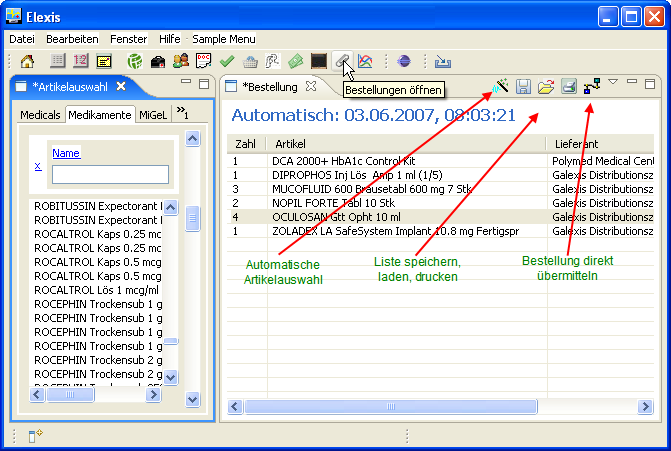
\includegraphics[width=0.9\textwidth]{images/bestell1}
  \caption{Bestellungen - View}
  \label{fig:bestellungen}
\end{center}
\end{figure}


A gauche vous trouvez la fenêtre déjà connue avec la liste de sélection d'article qui contient
toutes les catégories d'articles pour lesquels vous avez des Plugins (normalement pour des médicaments, Medicals, MiGel et des produits propres). 
A droite se trouve le champ pour les commandes qui est d'abord vide. Vous avez donc les possibilités suivantes :

\begin{itemize}
  \item En cliquant sur le symbole de la baguette magique tout les articles dont la quantité est tombée sous la limite de stock prédéfinie par vous seront automatiquement ajoutés à la commande. La commande contiendra autant d'article pour pouvoir atteindre le stock maximal prédéfini pour cet article spécifique.
  \item Depuis la fenêtre gauche vous pouvez aussi tirer un article vers la commande à droite.
	\item En cliquant sur la touche droite de la souris vous pouvez effacer un article de la liste de commande ou changer le chiffre de la quantité commandée.
	\item Vous pouvez sauvegarder d'abord une commande pour l'adapter plus tard. 
	
	\item Vous pouvez recharger des anciennes commandes pour les modifier.
	\item Vous pouvez imprimer les commandes. Pour cela il vous faut un modèle de texte du système (cf page
	\pageref{textvorlagen}) nommée  \glqq commande\grqq{} qui contient à un endroit spécifique un caractère de remplacement  [commande] (cf Fig. \ref{fig:bestell2}).
	\item Last but not least vous pouvez envoyer votre commande par Internet ou modem si vous possédez un Plugin spécifique pour votre livreur. Un Plugin existe déjà pour Galexis et d'autres sont en voie de développement.
\end{itemize}
\begin{figure}[hb]
  % Requires \usepackage{graphicx}
  
\includegraphics{images/bestell2}\\
  \caption{Ausschnitt aus der Vorlage Bestellung}\label{fig:bestell2}
\end{figure}

%\subsection{codes}
%Codes



